\begin{flushright} {\tiny {\color{gray} dgfem2D\_q1.tex}} \end{flushright}
%~~~~~~~~~~~~~~~~~~~~~~~~~~~~~~~~~~~~~~~~~~~~~~~~~~~~~~~~~~~~~~~~~~~~~~~~~~~~~~~~~~~~~~~~~~~~~~~~~~


Let us start with ${\cal A}_e$ where we assume that $k$ is constant within an element:
\begin{eqnarray}
{\cal A}_{\Omega_e}&=&
\left(
\begin{array}{ccc}
{\bm E} & {\bm 0} & {\bm H}_x \\
{\bm 0} & {\bm E} & {\bm H}_y \\
{\bm J}_x & {\bm J}_y & {\bm 0}
\end{array}
\right)
=
\left(
\begin{array}{ccc}
{\bm E} & {\bm 0} & -k_e{\bm J}_x \\
{\bm 0} & {\bm E} & -k_e{\bm J}_y \\
{\bm J}_x & {\bm J}_y & {\bm 0}
\end{array}
\right)
\end{eqnarray}
The matrices ${\bm E}$, ${\bm H}_x$, and ${\bm H}_y$ 
have been analytically derived in Appendix~\ref{app:qrle}:
\begin{scriptsize}
\[
{\bm E}=
\frac{h_x h_y}{9}
\left(
\begin{array}{cccc}
1 & 1/2 & 1/4 & 1/2 \\ 
1/2 & 1   & 1/2 & 1/4 \\ 
1/4 & 1/2 & 1 & 1/2 \\ 
1/2 & 1/4 & 1/2 & 1  
\end{array}
\right)
\qquad
{\bm J}_x=
\frac{h_y}{12} 
\left(
\begin{array}{cccc}
-2 & -2 & -1 & -1 \\
 2 &  2 &  1 & 1 \\
  1 &   1 & 2 & 2 \\
- 1 &  - 1 & -2 & -2
\end{array}
\right)
\qquad
{\bm J}_y=
\frac{h_x}{12} 
\left(
\begin{array}{cccc}
-2 & -1 & -1 & -2 \\
-1 & -2 & -2 & -1  \\
 1 &  2 &  2 &  1  \\
2 & 1 & 1 & 2 
\end{array}
\right) 
\]
\end{scriptsize}
The matrix ${\cal A}_{\Omega_e}$ is therefore trivial to implement. 

Let us now turn to $ {\cal A}_{\partial\Omega}$ which is specific to the DG method.
Because elements are rectangles then $n_i^+n_j^+=0$ if $i \neq j$ (where $i$ and $j$ 
are edge indices). 
Also, if $i=j$ then $n_i^+n_j^+=1$. 

\begin{center}
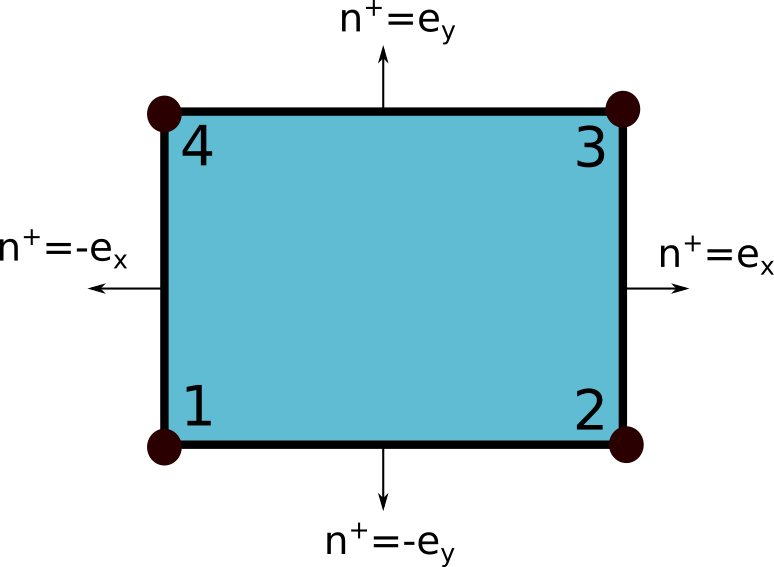
\includegraphics[width=7cm]{images/dgfem/dgelts_q1}
\end{center}

Assuming here again that heat conductivities are constant inside an element
it then follows that 
\begin{eqnarray}
 {\cal A}_{\partial\Omega_e}
&=&
\sum_{i=1}^{nedges}
\left(
\begin{array}{ccc}
{\bm E}_{xx,i} & {\bm E}_{xy,i} & {\bm H}_{x,i} \\
{\bm E}_{yx,i} & {\bm E}_{yy,i} & {\bm H}_{y,i} \\
{\bm J}_{x,i} & {\bm J}_{y,i} & {\bm G}_{T,i}
\end{array}
\right)
=
\sum_{i=1}^{nedges}
\left(
\begin{array}{ccc}
{\bm E}_{xx,i} & {\bm 0} & {\bm H}_{x,i} \\
{\bm 0} & {\bm E}_{yy,i} & {\bm H}_{y,i} \\
{\bm J}_{x,i} & {\bm J}_{y,i} & {\bm G}_{T,i}
\end{array}
\right)
\end{eqnarray}



Note that 
\begin{itemize}
\item $i=1$: bottom edge, i.e. $s=-1$ and then $N_4=N_3=0$; Also $\vec{n}_x^+=0$, $\vec{n}_y^+=-1$
\item $i=2$: right  edge, i.e.  $r=+1$ and then $N_1=N_4=0$; Also $\vec{n}_x^+=1$, $\vec{n}_y^+=0$
\item $i=3$: top edge, i.e. $s=+1$  and then $N_1=N_2=0$; Also $\vec{n}_x^+=0$, $\vec{n}_y^+=1$
\item $i=4$: left edge, i.e. $r=-1$ and then $N_2=N_3=0$; Also $\vec{n}_x^+=-1$, $\vec{n}_y^+=0$
\end{itemize}

Then 
\begin{eqnarray}
{\bm G}_{T,1} &=& -{\cal{E}} \int_{\partial\Omega_1} \vec{N}^T \vec{N} dS = -  {\cal{E}} {\bm C}_1 \nn\\
{\bm G}_{T,2} &=& -{\cal{E}} \int_{\partial\Omega_2} \vec{N}^T \vec{N} dS = -  {\cal{E}} {\bm C}_2 \nn\\
{\bm G}_{T,3} &=& -{\cal{E}} \int_{\partial\Omega_3} \vec{N}^T \vec{N} dS = -  {\cal{E}} {\bm C}_3 \nn\\
{\bm G}_{T,4} &=& -{\cal{E}} \int_{\partial\Omega_4} \vec{N}^T \vec{N} dS = -  {\cal{E}} {\bm C}_4 \nn
\end{eqnarray}
where the matrices ${\bm C}_i$ have been worked out in detail in appendix~\ref{app:qrle}:
\begin{eqnarray}
{\bm C}_{1} 
&=& \int_{1\rightarrow 2} \vec{N}^T \vec{N} dS  
=
\frac{h_x}{6}
\left(\begin{array}{cccc}
2 & 1 & 0 & 0 \\
1 & 2 & 0 & 0 \\
0 & 0 & 0 & 0 \\
0 & 0 & 0 & 0 
\end{array}\right)
\nn\\
\nn\\
{\bm C}_{2} 
&=& \int_{2\rightarrow 3} \vec{N}^T \vec{N} dS  
=
\frac{h_y}{6}
\left(\begin{array}{cccc}
0 & 0 & 0 & 0 \\
0 & 2 & 1 & 0 \\
0 & 1 & 2 & 0 \\
0 & 0 & 0 & 0 
\end{array}\right)
\nn\\
{\bm C}_{3}
&=& \int_{3\rightarrow 4} \vec{N}^T \vec{N} dS 
=
\frac{h_x}{6}
\left(\begin{array}{cccc}
0 & 0 & 0 & 0 \\
0 & 0 & 0 & 0 \\
0 & 0 & 2 & 1 \\
0 & 0 & 1 & 2 
\end{array}\right)
\nn\\
\nn\\
{\bm C}_{4} 
&=& \int_{4\rightarrow 1} \vec{N}^T \vec{N} dS  
=
\frac{h_y}{6}
\left(\begin{array}{cccc}
2 & 0 & 0 & 1 \\
0 & 0 & 0 & 0 \\
0 & 0 & 0 & 0 \\
1& 0 & 0 & 2 
\end{array}\right)
\nn
\end{eqnarray}

\begin{eqnarray}
{\bm E}_{xx,1} &=& -k_e {\cal F} \int_{\partial\Omega_1}  \vec{N}^T\vec{N}  {n}^+_x   n^+_x dS = 0 \nn\\ 
{\bm E}_{xx,2} &=& -k_e {\cal F} \int_{\partial\Omega_2}  \vec{N}^T\vec{N}  {n}^+_x   n^+_x dS = -k_e {\cal F} {\bm C}_2  \nn\\ 
{\bm E}_{xx,3} &=& -k_e {\cal F} \int_{\partial\Omega_3}  \vec{N}^T\vec{N}  {n}^+_x   n^+_x dS = 0 \nn\\ 
{\bm E}_{xx,4} &=& -k_e {\cal F} \int_{\partial\Omega_4}  \vec{N}^T\vec{N}  {n}^+_x   n^+_x dS = -k_e {\cal F} {\bm C}_4  
\nn\\
{\bm E}_{yy,1} &=& -k_e {\cal F} \int_{\partial\Omega_1}  \vec{N}^T\vec{N}  {n}^+_y   n^+_y dS = -k_e {\cal F} {\bm C}_1  \nn\\ 
{\bm E}_{yy,2} &=& -k_e {\cal F} \int_{\partial\Omega_2}  \vec{N}^T\vec{N}  {n}^+_y   n^+_y dS = 0 \nn\\ 
{\bm E}_{yy,3} &=& -k_e {\cal F} \int_{\partial\Omega_3}  \vec{N}^T\vec{N}  {n}^+_y   n^+_y dS = -k_e {\cal F} {\bm C}_3  \nn\\  
{\bm E}_{yy,4} &=& -k_e {\cal F} \int_{\partial\Omega_4}  \vec{N}^T\vec{N}  {n}^+_y   n^+_y dS = 0 
\nn\\ 
{\bm H}_{x,1} &=& k_e \int_{\partial\Omega_1}  \left( \frac{1}{2} + \vec{\cal C} \cdot \vec{n}^+ \right) \vec{N}^T \vec{N} n^+_x dS = 0 \nn\\ 
{\bm H}_{x,2} &=& k_e \int_{\partial\Omega_2}  \left( \frac{1}{2} + \vec{\cal C} \cdot \vec{n}^+ \right) \vec{N}^T \vec{N} n^+_x dS = k_e  \left( \frac{1}{2} + {\cal C}_x \right) {\bm C}_{2} \nn\\ 
{\bm H}_{x,3} &=& k_e \int_{\partial\Omega_3}  \left( \frac{1}{2} + \vec{\cal C} \cdot \vec{n}^+ \right) \vec{N}^T \vec{N} n^+_x dS = 0 \nn\\ 
{\bm H}_{x,4} &=& k_e \int_{\partial\Omega_4}  \left( \frac{1}{2} + \vec{\cal C} \cdot \vec{n}^+ \right) \vec{N}^T \vec{N} n^+_x dS = - k_e  \left( \frac{1}{2} - {\cal C}_x \right) {\bm C}_{4} 
\nn\\
{\bm H}_{y,1} &=& k_e \int_{\partial\Omega_1}  \left( \frac{1}{2} + \vec{\cal C} \cdot \vec{n}^+ \right) \vec{N}^T \vec{N} n^+_y dS = -k_e  \left( \frac{1}{2} - {\cal C}_y \right) {\bm C}_{1} \nn\\ 
{\bm H}_{y,2} &=& k_e \int_{\partial\Omega_2}  \left( \frac{1}{2} + \vec{\cal C} \cdot \vec{n}^+ \right) \vec{N}^T \vec{N} n^+_y dS = 0 \nn\\ 
{\bm H}_{y,3} &=& k_e \int_{\partial\Omega_3}  \left( \frac{1}{2} + \vec{\cal C} \cdot \vec{n}^+ \right) \vec{N}^T \vec{N} n^+_y dS = k_e  \left( \frac{1}{2} + {\cal C}_y \right) {\bm C}_{3} \nn\\ 
{\bm H}_{y,4} &=& k_e \int_{\partial\Omega_4}  \left( \frac{1}{2} + \vec{\cal C} \cdot \vec{n}^+ \right) \vec{N}^T \vec{N} n^+_y dS = 0 \nn\\ 
\nn\\
{\bm J}_{x,1} &=& \int_{\partial\Omega_1}  \left(\frac{1}{2} - \vec{\cal{C}} \cdot \vec{n}^+ \right) \vec{N}^T \vec{N} n^+_x  \; dS = 0 \nn\\ 
{\bm J}_{x,2} &=& \int_{\partial\Omega_2}  \left(\frac{1}{2} - \vec{\cal{C}} \cdot \vec{n}^+ \right) \vec{N}^T \vec{N} n^+_x  \; dS = \left(\frac{1}{2} - {\cal C}_x \right) {\bm C}_{2} \nn\\
{\bm J}_{x,3} &=& \int_{\partial\Omega_3}  \left(\frac{1}{2} - \vec{\cal{C}} \cdot \vec{n}^+ \right) \vec{N}^T \vec{N} n^+_x  \; dS = 0 \nn\\
{\bm J}_{x,4} &=& \int_{\partial\Omega_4}  \left(\frac{1}{2} - \vec{\cal{C}} \cdot \vec{n}^+ \right) \vec{N}^T \vec{N} n^+_x  \; dS = -\left(\frac{1}{2} + {\cal C}_x \right) {\bm C}_{4} \nn\\
\nn\\
{\bm J}_{y,1} &=& \int_{\partial\Omega_1}  \left(\frac{1}{2} - \vec{\cal{C}} \cdot \vec{n}^+ \right) \vec{N}^T \vec{N} n^+_y  \; dS = - \left(\frac{1}{2} + {\cal C}_y \right) {\bm C}_{1} \nn\\
{\bm J}_{y,2} &=& \int_{\partial\Omega_2}  \left(\frac{1}{2} - \vec{\cal{C}} \cdot \vec{n}^+ \right) \vec{N}^T \vec{N} n^+_y  \; dS = 0 \nn\\
{\bm J}_{y,3} &=& \int_{\partial\Omega_3}  \left(\frac{1}{2} - \vec{\cal{C}} \cdot \vec{n}^+ \right) \vec{N}^T \vec{N} n^+_y  \; dS =   \left(\frac{1}{2} - {\cal C}_y \right) {\bm C}_{3} \nn\\
{\bm J}_{y,4} &=& \int_{\partial\Omega_4}  \left(\frac{1}{2} - \vec{\cal{C}} \cdot \vec{n}^+ \right) \vec{N}^T \vec{N} n^+_y  \; dS = 0 \nn
\end{eqnarray}













